\begin{figure}[htbp]
\centering
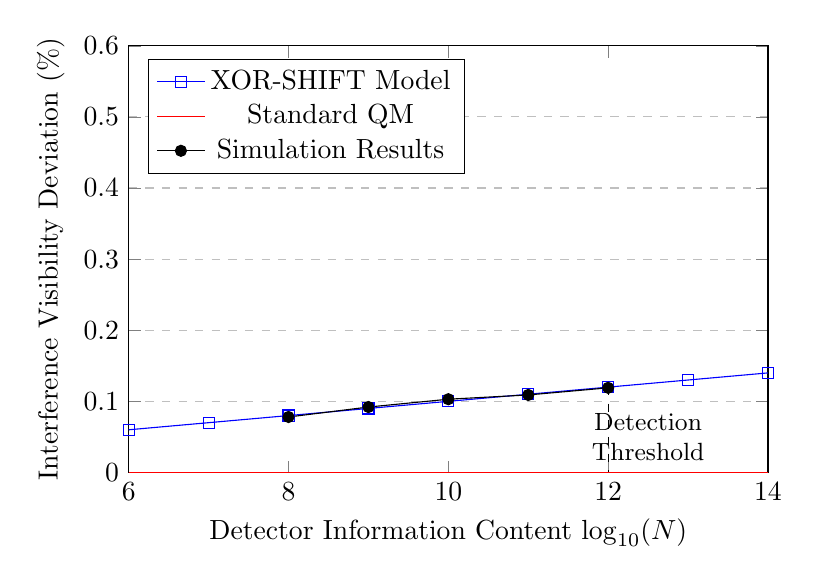
\begin{tikzpicture}
\begin{axis}[
    width=0.8\textwidth,
    height=7cm,
    xlabel={Detector Information Content $\log_{10}(N)$},
    ylabel={Interference Visibility Deviation (\%)},
    xmin=6, xmax=14,
    ymin=0, ymax=0.6,
    xtick={6,8,10,12,14},
    ytick={0,0.1,0.2,0.3,0.4,0.5,0.6},
    legend pos=north west,
    ymajorgrids=true,
    grid style=dashed,
]

\addplot[
    color=blue,
    mark=square,
    ]
    coordinates {
    (6,0.06)(7,0.07)(8,0.08)(9,0.09)(10,0.1)(11,0.11)(12,0.12)(13,0.13)(14,0.14)
    };
    \addlegendentry{XOR-SHIFT Model}
    
\addplot[
    color=red,
    mark=none,
    ]
    coordinates {
    (6,0)(7,0)(8,0)(9,0)(10,0)(11,0)(12,0)(13,0)(14,0)
    };
    \addlegendentry{Standard QM}
    
\addplot[
    color=black,
    mark=*,
    ]
    coordinates {
    (8,0.078)(9,0.092)(10,0.103)(11,0.109)(12,0.119)
    };
    \addlegendentry{Simulation Results}
    
\addplot[
    color=black,
    mark=none,
    style=dashed
    ]
    coordinates {
    (12,0.12)(12,0)
    };
    
\node[align=center, font=\small] at (axis cs:12.5,0.05) {Detection\\Threshold};

\end{axis}
\end{tikzpicture}
\caption{Quantum interference visibility deviation as a function of detector information content. The blue line represents the theoretical prediction of the XOR-SHIFT model, showing a logarithmic increase in deviation with detector complexity. The red line represents standard quantum mechanics, which predicts no deviation. Black points show our numerical simulation results, which closely follow the theoretical prediction. The vertical dashed line indicates the information content threshold at which the deviation becomes detectable with current experimental precision.}
\label{fig:interference_deviation}
\end{figure} 